% Conference: JCSSE 2026
%
% Compile (Overleaf): pdflatex slides_uhap.tex
%
% Upload these files next to this .tex on Overleaf (in a figures/ folder):
%   figures/system_architecture.png
%   figures/fig2_namespace_isolation.png
%   figures/fig3_permodel_latency.png
%   figures/fig5_update_latency.png

\documentclass[aspectratio=169,10pt]{beamer}

% ── Theme reset ─────────────────────────────────────────────────────────────
\usetheme{default}
\usecolortheme{default}
\setbeamertemplate{navigation symbols}{}

% ── Packages ────────────────────────────────────────────────────────────────
\usepackage[T1]{fontenc}
\IfFileExists{lmodern.sty}{\usepackage{lmodern}}{}
\usepackage[utf8]{inputenc}
\usepackage[expansion=false]{microtype}
\usepackage[table]{xcolor}
\usepackage{tikz}
\usetikzlibrary{calc,positioning,backgrounds,shapes.geometric,arrows.meta,fit}
\usepackage{tcolorbox}
\tcbuselibrary{skins}
\usepackage{booktabs}
\usepackage{array}
\usepackage{makecell}
\usepackage{amsmath,amssymb}
\usepackage{multirow}
\usepackage{graphicx}

% ── U-HAP palette ───────────────────────────────────────────────────────────
\definecolor{uhapNavy}{HTML}{0E2A4A}
\definecolor{uhapNavyD}{HTML}{081A30}
\definecolor{uhapTeal}{HTML}{00897B}
\definecolor{uhapTealD}{HTML}{00695C}
\definecolor{uhapAmber}{HTML}{FFF8E1}
\definecolor{uhapAmberBorder}{HTML}{F57F17}
\definecolor{uhapGray}{HTML}{F5F5F5}
\definecolor{uhapGrayD}{HTML}{546E7A}
\definecolor{uhapGreen}{HTML}{2E7D32}
\definecolor{uhapRed}{HTML}{C62828}

% ── Sans-serif throughout ───────────────────────────────────────────────────
\renewcommand{\familydefault}{\sfdefault}

% ── Beamer font sizes ───────────────────────────────────────────────────────
\setbeamercolor{normal text}{fg=uhapNavyD}
\setbeamercolor{frametitle}{fg=white,bg=uhapNavy}
\setbeamercolor{title}{fg=white}
\setbeamercolor{subtitle}{fg=uhapTeal}
\setbeamercolor{itemize item}{fg=uhapTeal}
\setbeamercolor{itemize subitem}{fg=uhapTeal}
\setbeamercolor{itemize subsubitem}{fg=uhapTeal}
\setbeamerfont{frametitle}{size=\large,series=\bfseries}
\setbeamerfont{itemize/enumerate body}{size=\scriptsize}
\setbeamerfont{itemize/enumerate subbody}{size=\tiny}

\setbeamertemplate{itemize item}{\color{uhapTeal}\textbullet}
\setbeamertemplate{itemize subitem}{\color{uhapTeal}\textendash}
\setbeamertemplate{itemize subsubitem}{\color{uhapTeal}$\circ$}

\newcommand{\tightitems}{%
  \setlength{\topsep}{1pt}%
  \setlength{\itemsep}{2pt}%
  \setlength{\parsep}{0pt}%
  \setlength{\parskip}{0pt}%
}

% ── Frame title bar ─────────────────────────────────────────────────────────
\setbeamertemplate{frametitle}{%
  \nointerlineskip
  \begin{beamercolorbox}[wd=\paperwidth,ht=1.0cm,dp=0cm,sep=0pt]{frametitle}%
    \vbox to 1.0cm{%
      \vfil
      \hbox{\hspace{0.45cm}\usebeamerfont{frametitle}\insertframetitle}%
      \vfil
    }%
  \end{beamercolorbox}%
}

% ── Footer bar ──────────────────────────────────────────────────────────────
\setbeamercolor{footer}{bg=uhapNavy,fg=white}
\setbeamertemplate{footline}{%
  \leavevmode
  \begin{beamercolorbox}[wd=\paperwidth,ht=0.42cm,dp=0.25cm,sep=0pt]{footer}%
    \hbox to \paperwidth{%
      \hspace{0.45cm}%
      \color{white}\tiny U-HAP: Unified Authorization over Heterogeneous Policies%
      \hfill%
      \color{white}\tiny\insertframenumber/\inserttotalframenumber%
      \hspace{0.45cm}%
    }%
  \end{beamercolorbox}%
}

% ── Compact callout box ──────────────────────────────────────────────────────
\newtcolorbox{callout}[2][]{%
  enhanced,
  colback=white,
  colframe=uhapNavy!18,
  coltitle=white,
  colbacktitle=uhapNavy,
  fonttitle=\bfseries\tiny,
  fontupper=\tiny,
  arc=1mm,outer arc=1mm,
  boxrule=0.4pt,titlerule=0pt,
  left=3pt,right=3pt,top=2pt,bottom=2pt,
  toptitle=1pt,bottomtitle=1pt,
  title={#2},#1
}

% ── Highlight banner ─────────────────────────────────────────────────────────
\newcommand{\highlightbanner}[1]{%
  \begin{center}
  \begin{tcolorbox}[colback=uhapGray,colframe=uhapGray,
                    boxrule=0pt,arc=1mm,
                    left=6pt,right=6pt,top=1pt,bottom=1pt,
                    width=0.97\linewidth,
                    borderline west={2pt}{0pt}{uhapTeal}]
  \tiny\color{uhapNavyD}#1
  \end{tcolorbox}
  \end{center}}

% ── Phase pill ───────────────────────────────────────────────────────────────
\newcommand{\phasepill}[1]{%
  \tcbox[colback=uhapAmber,colframe=uhapAmberBorder,boxrule=0.3pt,arc=1mm,
         left=3pt,right=3pt,top=0pt,bottom=0pt,on line,nobeforeafter]{%
    \tiny\color{uhapNavyD}\textbf{#1}}%
}

% ── Title/divider backgrounds ────────────────────────────────────────────────
\newcommand{\titleBg}{%
  \begin{tikzpicture}[overlay,remember picture]
    \fill[uhapNavy] (current page.south west) rectangle (current page.north east);
    \fill[uhapTeal]
      ([xshift=-1.6cm,yshift=0cm]current page.north east) circle (1.85cm);
    \fill[uhapNavy]
      ([xshift=-0.05cm,yshift=0cm]current page.north east) circle (1.85cm);
  \end{tikzpicture}%
}
\newcommand{\dividerBg}{%
  \begin{tikzpicture}[overlay,remember picture]
    \fill[uhapNavy] (current page.south west) rectangle (current page.north east);
    \fill[uhapTeal]
      ([xshift=-1.5cm,yshift=-0.5cm]current page.north east)
      rectangle ++(0.85cm,0.85cm);
  \end{tikzpicture}%
}

\graphicspath{{figures/}{./}{../figures/}}

\begin{document}

% ════════════════════════════════════════════════════════════════════════════
% 1. TITLE
% ════════════════════════════════════════════════════════════════════════════
\begin{frame}[plain,noframenumbering]
\titleBg
\vspace{1.1cm}\hspace{0.5cm}%
\begin{minipage}{0.85\paperwidth}
{\fontsize{34pt}{38pt}\selectfont\bfseries\color{white}U-HAP}\\[10pt]
{\fontsize{11pt}{14pt}\selectfont\bfseries\color{white}%
  Unified Authorization over Heterogeneous Policies}\\
{\fontsize{11pt}{14pt}\selectfont\bfseries\color{white}%
  with Efficient Multi-Resource Verification in Kubernetes}\\[7pt]
{\fontsize{9pt}{11pt}\selectfont\color{uhapTeal}JCSSE 2026 \textbullet{} Conference Paper Presentation}\\[20pt]
{\footnotesize\color{white}Krittapak Jairak \enspace Singha Junchan \enspace Phisitphon Pruksorranan}\\[3pt]
{\small\color{white}Advisor: Asst.\ Prof.\ Dr.\ Somchart Fugkeaw}\\[5pt]
{\small\color{white}School of ICT, SIIT, Thammasat University, Thailand}
\end{minipage}
\end{frame}

% ════════════════════════════════════════════════════════════════════════════
% 1b. BACKGROUND / INTRODUCTION  (SSO + Access Control in Kubernetes)
% ════════════════════════════════════════════════════════════════════════════
\begin{frame}[t]{Background: SSO and Access Control in Kubernetes}
\vspace{-13pt}
\begin{columns}[T,onlytextwidth]
\begin{column}{0.49\textwidth}
\begin{callout}[fonttitle=\bfseries\small,fontupper=\scriptsize]{Access Control in Kubernetes}
Post-authentication, every API call is dispatched as a \texttt{SubjectAccessReview} (SAR) to an \textbf{authorization phase}.
\begin{itemize}\tightitems
\item Built-in modes: \textbf{RBAC} (default), ABAC, Node, \textbf{Webhook}
\item \textbf{Webhook authorizer} delegates to an external service --- where \textbf{U-HAP} plugs in
\item Native RBAC lacks fine-grained, \emph{context-aware} authorization
\end{itemize}
\end{callout}
\vspace{0pt}
\begin{callout}[fontupper=\scriptsize]{Access-Control Models in Practice}
\setlength{\tabcolsep}{3pt}\renewcommand{\arraystretch}{1.05}
\begin{tabular}{@{}>{\scriptsize\bfseries\color{uhapNavy}}l >{\scriptsize}p{4.35cm}@{}}
RBAC & grant access by assigning \emph{roles} to users \\
ABAC & grant access via \emph{attribute conditions} \\
ACL  & explicit \emph{list} of allowed users / groups \\
Deny & explicit block; \emph{overrides} any allow \\
\end{tabular}
\end{callout}
\end{column}
\begin{column}{0.49\textwidth}
\begin{callout}[fonttitle=\bfseries\small,fontupper=\scriptsize]{Single Sign-On (SSO)}
SSO lets a user authenticate \emph{once} with a single identity (e.g.\ OIDC / Keycloak) and reuse it across many services.
\begin{itemize}\tightitems
\item Solves \textbf{authentication} --- \emph{who you are}
\item Does \emph{not} solve \textbf{authorization} --- \emph{what you may do}
\item After SSO, each resource still enforces \emph{its own} policy model independently
\end{itemize}
\end{callout}
\vspace{1pt}
\begin{center}
\scalebox{0.92}{%
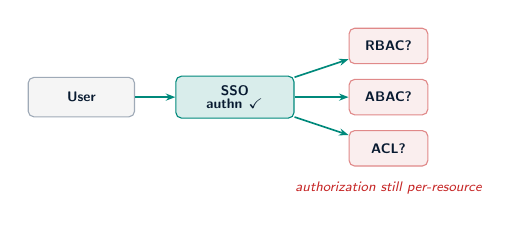
\begin{tikzpicture}[
  b/.style={draw=uhapNavy!40,fill=uhapGray,rounded corners=2pt,
            minimum width=1.35cm,minimum height=0.5cm,
            font=\tiny\bfseries,text=uhapNavyD,align=center},
  ok/.style={draw=uhapTeal,fill=uhapTeal!15,rounded corners=2pt,
             minimum width=1.5cm,minimum height=0.5cm,
             font=\tiny\bfseries,text=uhapNavyD,align=center},
  pol/.style={draw=uhapRed!55,fill=uhapRed!8,rounded corners=2pt,
              minimum width=1.0cm,minimum height=0.45cm,
              font=\tiny\bfseries,text=uhapNavyD,align=center},
  a/.style={-{Stealth[scale=0.6]},uhapTeal,semithick}]
  \node[b]  (u)  at (0,0)      {User};
  \node[ok] (sso)at (1.95,0)   {SSO\\[-1pt]{\tiny authn \checkmark}};
  \node[pol](r)  at (3.9,0.65) {RBAC?};
  \node[pol](ab) at (3.9,0)    {ABAC?};
  \node[pol](ac) at (3.9,-0.65){ACL?};
  \draw[a] (u)--(sso);
  \draw[a] (sso)--(r); \draw[a] (sso)--(ab); \draw[a] (sso)--(ac);
  \node[font=\tiny\itshape,text=uhapRed,align=center] at (3.9,-1.15)
    {authorization still per-resource};
\end{tikzpicture}}
\end{center}
\vspace{1pt}
\highlightbanner{SSO unifies \emph{login}; it leaves \emph{authorization} fragmented across RBAC, ABAC, and ACL. U-HAP unifies the authorization side.}
\end{column}
\end{columns}
\end{frame}

% ════════════════════════════════════════════════════════════════════════════
% 1c. RELATED WORK
% ════════════════════════════════════════════════════════════════════════════
\begin{frame}[t]{Related Work and Its Limitations}
\vspace{2pt}
\begin{columns}[T,onlytextwidth]
\begin{column}{0.49\textwidth}
\begin{callout}[fonttitle=\bfseries\scriptsize,fontupper=\tiny]{Hardening \& Misconfiguration}
\begin{itemize}\tightitems
\item NSA/CISA hardening guidance [1]; empirical misconfiguration studies [2,3]; EPScan detects excessive RBAC permissions [10]
\item Formal verification of access policies [11]
\end{itemize}
\emph{Limitation:} target \textbf{correctness of individual policies} --- not \emph{unified} authorization across mixed models.
\end{callout}
\vspace{2pt}
\begin{callout}[fonttitle=\bfseries\scriptsize,fontupper=\tiny]{RBAC, Policy-as-Code \& Zero Trust}
\begin{itemize}\tightitems
\item K8s RBAC [4]; Zero Trust architecture [12]; PerfSPEC profiling [13]; compile-time policy optimization [14]
\end{itemize}
\emph{Limitation:} operate \textbf{within a single model}; repeated per-layer evaluation $\Rightarrow$ redundant checks and added latency.
\end{callout}
\end{column}
\begin{column}{0.49\textwidth}
\begin{callout}[fonttitle=\bfseries\scriptsize,fontupper=\tiny]{Expressive \& Graph-Based Models}
\begin{itemize}\tightitems
\item XACML [7]: expressive but heavyweight PDP, ill-suited to low-latency cloud-native; compiled-XACML indices [15] motivate our compile-time design
\item Graph / relationship-based AC [8,16]; Zanzibar [17] scales but needs \emph{runtime graph traversal}; ABAC$\to$RBAC conversion [18]
\end{itemize}
\emph{Limitation:} heavy PDPs, runtime-traversal overhead, or interoperability only --- no efficient \emph{unified} runtime.
\end{callout}
\vspace{2pt}
\begin{callout}[fonttitle=\bfseries\scriptsize,fontupper=\scriptsize]{The Gap U-HAP Fills}
No prior work offers a \textbf{unified} framework spanning \textbf{RBAC + ABAC + ACL + deny} that minimizes redundant evaluation while guaranteeing \textbf{scalable, low-latency} multi-resource authorization.
\end{callout}
\end{column}
\end{columns}
\end{frame}

% ════════════════════════════════════════════════════════════════════════════
% 2. MOTIVATION
% ════════════════════════════════════════════════════════════════════════════
\begin{frame}[t]{Motivation: The Kubernetes Authorization Problem}
\vspace{3pt}
\begin{columns}[T,onlytextwidth]
\begin{column}{0.46\textwidth}
{\scriptsize\bfseries\color{uhapNavyD}Modern K8s deployments are \emph{multi-model}}\\[4pt]
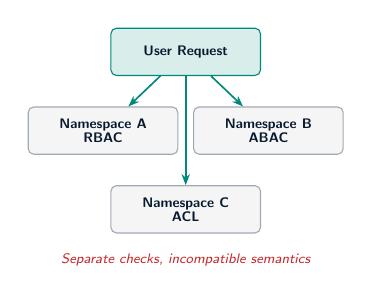
\begin{tikzpicture}[
  box/.style={draw=uhapNavy!40,fill=uhapGray,rounded corners=2pt,
              minimum width=1.9cm,minimum height=0.6cm,
              font=\tiny\bfseries,text=uhapNavyD,align=center},
  arrow/.style={-{Stealth[scale=0.7]},uhapTeal,semithick}]
  \node[box] (a) at (0,1.8)   {Namespace A\\[-1pt]{\tiny RBAC}};
  \node[box] (b) at (2.1,1.8) {Namespace B\\[-1pt]{\tiny ABAC}};
  \node[box] (c) at (1.05,0.8){Namespace C\\[-1pt]{\tiny ACL}};
  \node[box,fill=uhapTeal!15,draw=uhapTeal] (u) at (1.05,2.8)
                                            {User Request};
  \draw[arrow] (u) -- (a);
  \draw[arrow] (u) -- (b);
  \draw[arrow] (u) -- (c);
  \node[font=\tiny\itshape,text=uhapRed] at (1.05,0.15)
    {Separate checks, incompatible semantics};
\end{tikzpicture}
\vspace{4pt}
\setlength{\tabcolsep}{3pt}\renewcommand{\arraystretch}{1.2}
\begin{tabular}{@{}>{\tiny\bfseries\color{uhapNavy}}l >{\tiny}p{3.1cm}@{}}
RBAC & Role-Based: grant access by assigning \emph{roles} to users \\
ABAC & Attribute-Based: grant access via \emph{attribute conditions} \\
ACL  & Access Control List: explicit \emph{named list} of allowed users \\
\end{tabular}
\end{column}
\begin{column}{0.52\textwidth}
\begin{callout}[fonttitle=\bfseries\small,fontupper=\footnotesize]{Three Key Challenges}
\begin{itemize}\tightitems
\item \textbf{Semantic fragmentation} --- RBAC, ABAC, ACL use incompatible rule languages and evaluation semantics
\item \textbf{Non-deterministic conflicts} --- Implicit ordering across models yields inconsistent deny/allow decisions
\item \textbf{Runtime inefficiency} --- Repeated policy scans evaluate irrelevant rules for every request
\end{itemize}
\end{callout}
\vspace{3pt}
\begin{center}
\begin{tcolorbox}[colback=uhapGray,colframe=uhapGray,
                  boxrule=0pt,arc=1mm,
                  left=6pt,right=6pt,top=2pt,bottom=2pt,
                  width=0.97\linewidth,
                  borderline west={2pt}{0pt}{uhapTeal}]
\footnotesize\color{uhapNavyD}Even with SSO handling authentication, \emph{authorization across multiple resources remains fragmented, slow, and inconsistent}.
\end{tcolorbox}
\end{center}
\end{column}
\end{columns}
\end{frame}

% ════════════════════════════════════════════════════════════════════════════
% 3. OUR SOLUTION
% ════════════════════════════════════════════════════════════════════════════
\begin{frame}[t]{Our Solution: U-HAP}
\vspace{3pt}
\begin{columns}[T,onlytextwidth]
\begin{column}{0.49\textwidth}
\begin{callout}{Core Idea}
Shift expensive reasoning \emph{offline}. Compile all policy models into
\textbf{resource--action indexed artifacts} $C_{\langle n,r,a\rangle}$.
Every request-time authorization reduces to an O(1) index lookup followed
by cheap, model-specific index evaluation.
\end{callout}
\vspace{3pt}
\begin{callout}{Three-Phase Architecture}
\begin{itemize}\tightitems
\item \phasepill{Phase 1} Setup \& trust configuration (deploy-time)
\item \phasepill{Phase 2} Compilation: DSL parse $\to$ DAG $\to$ indexed artifacts (policy-change time)
\item \phasepill{Phase 3} Request eval: O(1) lookup $\to$ pruning $\to$ index eval (every SAR --- SubjectAccessReview)
\end{itemize}
\end{callout}
\end{column}
\begin{column}{0.49\textwidth}
\begin{callout}{Key Contributions}
\begin{itemize}\tightitems
\item \textbf{Universal semantic graph} capturing RBAC, ABAC, and ACL in a unified DAG (Directed Acyclic Graph) with deny-override semantics
\item \textbf{Hash consing}: structurally identical predicates share one node — 11 nodes reduced to 8 in our 4-policy example
\item \textbf{Two-level pruning}: policy-type pruning skips inactive model classes; token-driven pruning limits evaluation to relevant rules
\item \textbf{Deterministic conflict resolution}: deny-overrides-all, always, across all models
\end{itemize}
\end{callout}
\end{column}
\end{columns}
\end{frame}

% ════════════════════════════════════════════════════════════════════════════
% 4. SYSTEM ARCHITECTURE (merged)
% ════════════════════════════════════════════════════════════════════════════
\begin{frame}[t]{System Architecture: Three-Phase Design}
\vspace{-14pt}
\begin{columns}[T,onlytextwidth]
\begin{column}{0.62\textwidth}
\centering
\IfFileExists{figures/system_architecture.png}{%
  \includegraphics[width=\linewidth,height=0.62\textheight,keepaspectratio]%
    {figures/system_architecture.png}%
}{%
\scalebox{0.62}{%
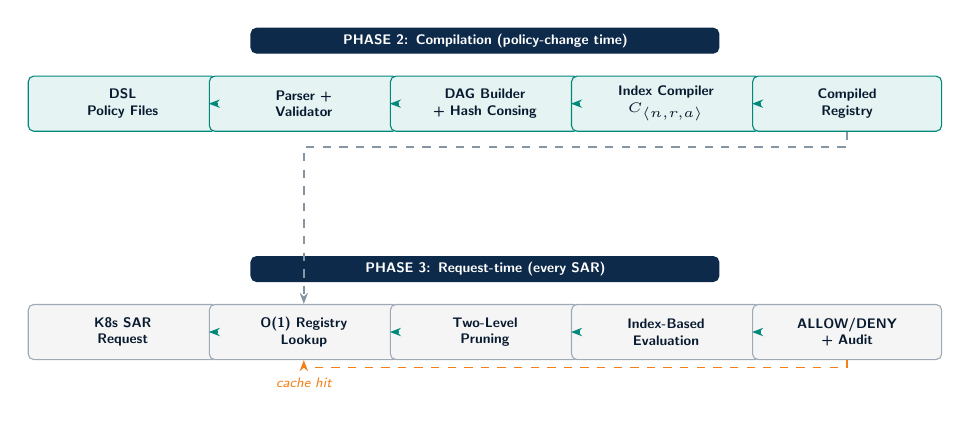
\begin{tikzpicture}[
  box/.style={draw=uhapNavy!40,fill=uhapGray,rounded corners=2pt,
              minimum width=2.4cm,minimum height=0.7cm,
              font=\tiny\bfseries,text=uhapNavyD,align=center},
  pbox/.style={draw=uhapTeal,fill=uhapTeal!10,rounded corners=2pt,
               minimum width=2.4cm,minimum height=0.7cm,
               font=\tiny\bfseries,text=uhapNavyD,align=center},
  arr/.style={-{Stealth[scale=0.7]},uhapTeal,semithick},
  lbl/.style={draw=uhapNavy,fill=uhapNavy,text=white,rounded corners=2pt,
              font=\tiny\bfseries,inner sep=2pt,text width=5.8cm,align=center}]
  \node[lbl] at (0,3.35) {PHASE 2: Compilation (policy-change time)};
  \node[pbox] (dsl)   at (-4.6,2.55) {DSL\\Policy Files};
  \node[pbox] (parse) at (-2.3,2.55) {Parser +\\Validator};
  \node[pbox] (dag)   at (0,2.55)    {DAG Builder\\+ Hash Consing};
  \node[pbox] (idx)   at (2.3,2.55)  {Index Compiler\\$C_{\langle n,r,a\rangle}$};
  \node[pbox] (reg)   at (4.6,2.55)  {Compiled\\Registry};
  \draw[arr] (dsl)--(parse); \draw[arr] (parse)--(dag);
  \draw[arr] (dag)--(idx);   \draw[arr] (idx)--(reg);

  \node[lbl] at (0,0.45) {PHASE 3: Request-time (every SAR)};
  \node[box] (sar)    at (-4.6,-0.35) {K8s SAR\\Request};
  \node[box] (lookup) at (-2.3,-0.35) {O(1) Registry\\Lookup};
  \node[box] (prune)  at (0,-0.35)    {Two-Level\\Pruning};
  \node[box] (eval)   at (2.3,-0.35)  {Index-Based\\Evaluation};
  \node[box] (dec)    at (4.6,-0.35)  {ALLOW/DENY\\+ Audit};
  \draw[arr] (sar)--(lookup); \draw[arr] (lookup)--(prune);
  \draw[arr] (prune)--(eval); \draw[arr] (eval)--(dec);
  \draw[arr,dashed,uhapNavy!50] (reg) -- ++(0,-0.55) -| (lookup);
  \draw[arr,uhapAmberBorder,dashed] (dec) -- ++(0,-0.45)
        -| node[midway,below,font=\tiny\itshape]{cache hit} (lookup);
\end{tikzpicture}%
}%
}
\end{column}
\begin{column}{0.36\textwidth}
\begin{callout}[fontupper=\tiny]{Phase 1: Setup \textnormal{\tiny(deploy-time)}}
\begin{itemize}\tightitems
\item Load \& validate DSL policies
\item Init webhook; zero request-time cost
\end{itemize}
\end{callout}
\vspace{2pt}
\begin{callout}[fontupper=\tiny]{Phase 2: Compilation \textnormal{\tiny(per policy change)}}
\begin{itemize}\tightitems
\item Parse DSL $\to$ hash-consed DAG
\item Compile $C_{\langle n,r,a\rangle}$ indices per triple
\item Store artifacts in registry
\end{itemize}
\end{callout}
\vspace{2pt}
\begin{callout}[fontupper=\tiny]{Phase 3: Request-time \textnormal{\tiny(every SAR)}}
\begin{itemize}\tightitems
\item O(1) lookup on $(n,r,a)$
\item Two-level pruning skips inactive models
\item Eval: hash set / bit-vector / gates
\item Return ALLOW/DENY + audit log
\end{itemize}
\end{callout}
\end{column}
\end{columns}
\end{frame}

% ════════════════════════════════════════════════════════════════════════════
% 5. HASH CONSING + COMPILED INDICES
% ════════════════════════════════════════════════════════════════════════════
\begin{frame}[t]{Compilation: Hash Consing and Indexed Artifacts}
\vspace{-4pt}
\begin{columns}[T,onlytextwidth]
%% ── Left: visual diagram ────────────────────────────────────────────
\begin{column}{0.47\textwidth}
\centering
\scalebox{1.20}{%
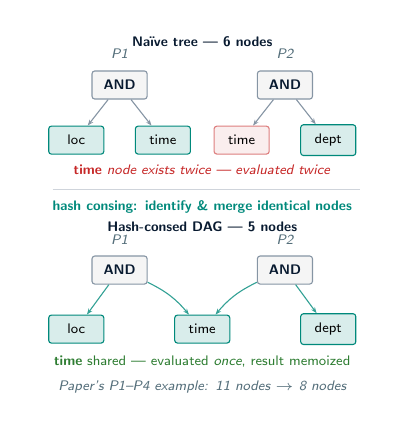
\begin{tikzpicture}[
  anode/.style={draw=uhapNavy!50,fill=uhapGray,rounded corners=1pt,
                font=\tiny\bfseries,text=uhapNavyD,
                minimum width=0.7cm,minimum height=0.33cm},
  snode/.style={draw=uhapTeal,fill=uhapTeal!15,rounded corners=1pt,
                font=\tiny,minimum width=0.7cm,minimum height=0.30cm},
  dnode/.style={draw=uhapRed!60,fill=uhapRed!8,rounded corners=1pt,
                font=\tiny,minimum width=0.7cm,minimum height=0.30cm},
  arr/.style={-{Stealth[scale=0.45]},uhapNavy!50,thin},
  tarr/.style={-{Stealth[scale=0.45]},uhapTeal!80,thin}]

%% Naïve tree (top)
\node[font=\tiny\bfseries,color=uhapNavyD,text width=4cm,align=center]
  at (1.8,4.1) {Naïve tree --- \textbf{6 nodes}};

\node[anode] (na1) at (0.75,3.55) {AND};
\node[anode] (na2) at (2.85,3.55) {AND};
\node[font=\tiny\itshape,color=uhapGrayD] at (0.75,3.95) {P1};
\node[font=\tiny\itshape,color=uhapGrayD] at (2.85,3.95) {P2};

\node[snode] (nL)  at (0.2, 2.85) {loc};
\node[snode] (nT1) at (1.3, 2.85) {time};
\node[dnode] (nT2) at (2.3, 2.85) {time};
\node[snode] (nD)  at (3.4, 2.85) {dept};

\draw[arr] (na1)--(nL);  \draw[arr] (na1)--(nT1);
\draw[arr] (na2)--(nT2); \draw[arr] (na2)--(nD);

\node[font=\tiny,color=uhapRed,text width=4.2cm,align=center]
  at (1.8,2.48) {\textit{\textbf{time} node exists twice --- evaluated twice}};

%% Divider + label
\draw[uhapNavy!20,thin] (-0.1,2.22) -- (3.8,2.22);
\node[font=\tiny\bfseries,color=uhapTeal,text width=4cm,align=center]
  at (1.8,2.0) {hash consing: identify \& merge identical nodes};

%% Hash-consed DAG (bottom)
\node[font=\tiny\bfseries,color=uhapNavyD,text width=4cm,align=center]
  at (1.8,1.75) {Hash-consed DAG --- \textbf{5 nodes}};

\node[anode] (db1) at (0.75,1.2) {AND};
\node[anode] (db2) at (2.85,1.2) {AND};
\node[font=\tiny\itshape,color=uhapGrayD] at (0.75,1.58) {P1};
\node[font=\tiny\itshape,color=uhapGrayD] at (2.85,1.58) {P2};

\node[snode] (dL) at (0.2,  0.45) {loc};
\node[snode] (dT) at (1.8,  0.45) {time};
\node[snode] (dD) at (3.4,  0.45) {dept};

\draw[tarr] (db1)--(dL);
\draw[tarr] (db1) to[bend left=12] (dT);
\draw[tarr] (db2) to[bend right=12] (dT);
\draw[tarr] (db2)--(dD);

\node[font=\tiny,color=uhapGreen,text width=4.2cm,align=center]
  at (1.8,0.04) {\textbf{time} shared --- evaluated \emph{once}, result memoized};

\node[font=\tiny\itshape,color=uhapGrayD,text width=4.2cm,align=center]
  at (1.8,-0.28) {Paper's P1--P4 example: 11 nodes $\to$ 8 nodes};
\end{tikzpicture}%
}
\end{column}
%% ── Right: index table ──────────────────────────────────────────────
\begin{column}{0.51\textwidth}
\begin{callout}{What Hash Consing Gives You}
\begin{itemize}\tightitems
\item Identical sub-expressions across policies share \textbf{one DAG node}
\item Each node evaluated \emph{at most once} per request (memoized)
\item Structural equality check --- not string comparison
\item Cost grows sub-linearly as policies share predicates
\end{itemize}
\end{callout}
\vspace{0pt}
\begin{callout}{Compiled Indexed Artifacts $C_{\langle n,r,a\rangle}$}
{\tiny For each \texttt{(namespace, resource, action)} triple:}\vspace{1pt}

\setlength{\tabcolsep}{3pt}
\renewcommand{\arraystretch}{1.0}
\begin{tabular}{@{}l p{4.2cm}@{}}
$I_{\mathrm{deny}}$  & deny candidate set (token-pruned hash set) \\
$I_{\mathrm{acl}}$   & ACL user/group hash set (O(1) membership) \\
$b_{\mathrm{rbac}}$  & RBAC bit-vector (one AND with $b_{\mathrm{user}}$) \\
$I_{\mathrm{abac}}$  & ABAC gate list, cost-sorted, key-pruned \\
\end{tabular}\vspace{1pt}

\textbf{Runtime order:}
Cache $\to$ Deny $\to$ ACL $\to$ RBAC $\to$ ABAC $\to$ Default Deny
\end{callout}
\vspace{-1pt}
\highlightbanner{The DAG is a compile-time artifact only. No graph traversal at runtime --- pure index lookup.}
\end{column}
\end{columns}
\end{frame}

% ════════════════════════════════════════════════════════════════════════════
% 6. TWO-LEVEL PRUNING
% ════════════════════════════════════════════════════════════════════════════
\begin{frame}[t]{Two-Level Pruning Strategy}
\vspace{3pt}
\begin{columns}[T,onlytextwidth]
\begin{column}{0.49\textwidth}
\begin{callout}{Level 1 --- Policy-Type Pruning}
Skip entire model classes that cannot produce a decision for this request.
\begin{itemize}\tightitems
\item If no deny rules exist for \texttt{(n,r,a)}: skip deny phase
\item If no RBAC policies apply: skip bit-vector AND
\item If caller has no attributes: skip ABAC gate list
\end{itemize}
\end{callout}
\vspace{3pt}
\begin{callout}{Level 2 --- Token-Driven Pruning}
Restrict evaluation to rules matching the caller's token.
\begin{itemize}\tightitems
\item \textbf{ACL}: hash-set membership --- O(1), no scan
\item \textbf{RBAC}: $b_{\mathrm{user}}\ \&\ b_{\mathrm{rbac}} \neq 0$ (single bitwise AND)\\
      {\tiny\color{uhapGrayD} Each bit = one role. User has admin(bit 2)+viewer(bit 5):\\
      $b_{\rm user}$=\texttt{…100100}, policy needs admin: $b_{\rm rbac}$=\texttt{…000100}\\
      \texttt{AND} $\neq$ 0 $\Rightarrow$ \textcolor{uhapGreen}{\textbf{ALLOW}}. One operation regardless of role count.}
\item \textbf{ABAC}: attribute-key index narrows candidates before gate evaluation
\end{itemize}
\end{callout}
\end{column}
\begin{column}{0.49\textwidth}
\begin{callout}{Deny-Overrides-All Invariant}
\textbf{Deny is always checked first.} If any deny candidate matches the caller's token and request context, the decision is \texttt{DENY} --- regardless of any allow rules in ACL, RBAC, or ABAC.

This invariant is enforced at compile time and cannot be bypassed.
\end{callout}
\vspace{3pt}
\begin{callout}{Runtime Evaluation Pipeline}
\begin{center}
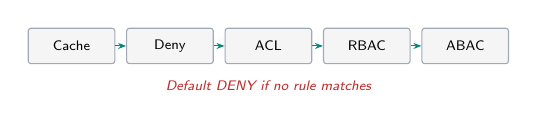
\begin{tikzpicture}[
  s/.style={draw=uhapNavy!40,fill=uhapGray,rounded corners=1pt,
            minimum width=1.1cm,minimum height=0.45cm,font=\tiny,align=center},
  a/.style={-{Stealth[scale=0.6]},uhapTeal}]
  \node[s] (c)   at (0,0)   {Cache};
  \node[s] (d)   at (1.25,0){Deny};
  \node[s] (acl) at (2.5,0) {ACL};
  \node[s] (rb)  at (3.75,0){RBAC};
  \node[s] (ab)  at (5.0,0) {ABAC};
  \draw[a](c)--(d);\draw[a](d)--(acl);\draw[a](acl)--(rb);\draw[a](rb)--(ab);
  \node[font=\tiny\itshape,text=uhapRed] at (2.5,-0.5){Default DENY if no rule matches};
\end{tikzpicture}
\end{center}
\end{callout}
\end{column}
\end{columns}
\end{frame}

% ════════════════════════════════════════════════════════════════════════════
% 7. EVALUATION SETUP
% ════════════════════════════════════════════════════════════════════════════
\begin{frame}[t]{Evaluation Setup}
\vspace{3pt}
\begin{columns}[T,onlytextwidth]
\begin{column}{0.49\textwidth}
\begin{callout}{Hardware and Implementation}
\begin{itemize}\tightitems
\item AMD Ryzen 9 7945HX (16C/32T), 32\,GB DDR5-4800, CachyOS Linux
\item U-HAP: Python 3.11 (in-memory evaluation)
\item Baseline: conventional SSO-based system performing sequential policy scanning
\end{itemize}
\end{callout}
\vspace{3pt}
\begin{callout}{Measurement Methodology}
\begin{itemize}\tightitems
\item Median of \textbf{1,000 iterations} after 50 warm-up runs
\item \textbf{In-memory policy lookup and verification only} --- no network, no auth overhead
\item Each namespace: 46 rules (10 RBAC, 20 ABAC, 10 ACL, 1 deny, 5 hierarchy edges)
\item ABAC gates: AND/OR/ATLEAST with ${\sim}50\%$ atom sharing across rules
\end{itemize}
\end{callout}
\end{column}
\begin{column}{0.49\textwidth}
\begin{callout}{Why In-Memory Benchmarks?}
\begin{itemize}\tightitems
\item Isolates \emph{pure algorithm cost} from network and framework overhead
\item Reveals true compilation gains: hash-consed DAG vs.\ sequential scan
\item Caching effect visible directly without HTTP round-trip noise
\end{itemize}
\end{callout}
\vspace{1pt}
\begin{callout}{Baseline: SSO-Based Sequential Evaluation}
\begin{itemize}\tightitems
\item Iterates over all policy rules per request
\item RBAC: repeated role resolution + hierarchy traversal at runtime
\item Represents conventional authorization without compile-time indexing
\end{itemize}
\end{callout}
\end{column}
\end{columns}
\end{frame}

% ════════════════════════════════════════════════════════════════════════════
% 8. EXPERIMENT 1 — APPLICATION SCALABILITY
% ════════════════════════════════════════════════════════════════════════════
\begin{frame}[t]{Experiment 1: Policy Verification Efficiency}
\vspace{-2pt}
\begin{columns}[T,onlytextwidth]
%% Left: graph + key results
\begin{column}{0.55\textwidth}
\centering
\IfFileExists{figures/fig2_namespace_isolation.png}{%
  \includegraphics[width=\linewidth,height=0.44\textheight,keepaspectratio]%
    {figures/fig2_namespace_isolation.png}%
}{%
  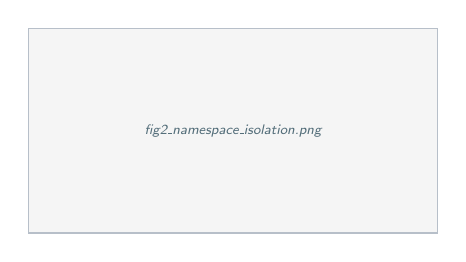
\begin{tikzpicture}
    \draw[fill=uhapGray,draw=uhapNavy!30] (0,0) rectangle (5.2,2.6);
    \node[font=\tiny\itshape,text=uhapGrayD] at (2.6,1.3){fig2\_namespace\_isolation.png};
  \end{tikzpicture}%
}
\vspace{2pt}
\begin{callout}[fontupper=\scriptsize]{Key Results}
\begin{itemize}\tightitems
\item \textbf{Isolation:} curves flat as $N{:}10{\to}1{,}000$ --- adding namespaces has \emph{zero} cost
\item \textbf{U-HAP:} ${\approx}$15.5\,\textmu s --- O(1) lookup, constant vs.\ $N$
\item \textbf{+Cache:} ${\approx}$1.8\,\textmu s --- \textbf{14--15$\times$} speedup over SSO
\item \textbf{SSO:} ${\approx}$26\,\textmu s --- 1.6--1.7$\times$ slower than U-HAP
\end{itemize}
\end{callout}
\end{column}
%% Right: vertical table
\begin{column}{0.43\textwidth}
{\tiny\textbf{Latency (\textmu s, median, 1\,000 iters)}}\\[1pt]
{\tiny 46 rules each: 10 RBAC + 20 ABAC + 10 ACL + 1 deny}
\vspace{3pt}
\setlength{\tabcolsep}{3pt}\renewcommand{\arraystretch}{1.15}
\begin{tabular}{@{}r rrr@{}}
\toprule
\tiny\textbf{N} & \tiny\textbf{U-HAP} & \tiny\textbf{+Cache} & \tiny\textbf{SSO} \\
\midrule
\tiny 10   & \tiny 15.6 & \tiny 1.7 & \tiny 26.9 \\
\tiny 50   & \tiny 15.4 & \tiny 1.8 & \tiny 26.0 \\
\tiny 100  & \tiny 15.5 & \tiny 1.8 & \tiny 25.8 \\
\tiny 200  & \tiny 15.6 & \tiny 1.7 & \tiny 25.2 \\
\tiny 300  & \tiny 15.4 & \tiny 1.8 & \tiny 26.4 \\
\tiny 500  & \tiny 15.6 & \tiny 1.8 & \tiny 26.0 \\
\tiny 750  & \tiny 15.7 & \tiny 1.7 & \tiny 25.4 \\
\tiny 1000 & \tiny 15.4 & \tiny 1.8 & \tiny 25.3 \\
\bottomrule
\end{tabular}
\end{column}
\end{columns}
\end{frame}

% ════════════════════════════════════════════════════════════════════════════
% 9. EXPERIMENT 2 — RULE DENSITY
% ════════════════════════════════════════════════════════════════════════════
\begin{frame}[t]{Experiment 2: Policy Size Impact}
\vspace{-2pt}
\begin{columns}[T,onlytextwidth]
%% Left: graph + key results
\begin{column}{0.55\textwidth}
\centering
\IfFileExists{figures/fig3_permodel_latency.png}{%
  \includegraphics[width=\linewidth,height=0.44\textheight,keepaspectratio]%
    {figures/fig3_permodel_latency.png}%
}{%
  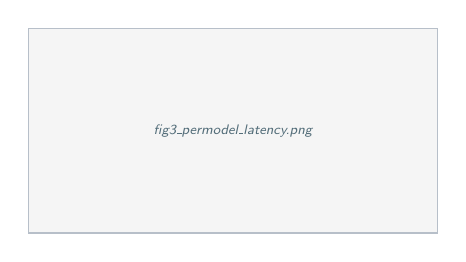
\begin{tikzpicture}
    \draw[fill=uhapGray,draw=uhapNavy!30] (0,0) rectangle (5.2,2.6);
    \node[font=\tiny\itshape,text=uhapGrayD] at (2.6,1.3){fig3\_permodel\_latency.png};
  \end{tikzpicture}%
}
\vspace{2pt}
\begin{callout}[fontupper=\scriptsize]{Key Results}
\begin{itemize}\tightitems
\item \textbf{ABAC:} hash-consed DAG → $\mathbf{16.9\times}$ at $k{=}320$; crossover $k{\approx}18$
\item \textbf{RBAC:} bit-vector AND → $\mathbf{5.6\times}$ at $k{=}320$; crossover $k{\approx}15$
\item \textbf{ACL:} hash-set → $\mathbf{5.0\times}$ at $k{=}320$; crossover $k{\approx}35$
\item $<$1$\times$ at small $k$: compilation overhead not yet amortized
\end{itemize}
\end{callout}
\end{column}
%% Right: vertical table
\begin{column}{0.43\textwidth}
{\tiny\textbf{Speedup vs.\ SSO baseline}}\\[1pt]
{\tiny $<$1$\times$ = compilation cost not yet amortized}
\vspace{3pt}
\setlength{\tabcolsep}{3pt}\renewcommand{\arraystretch}{1.15}
\begin{tabular}{@{}r rrr@{}}
\toprule
\tiny\textbf{k} & \tiny\textbf{ABAC} & \tiny\textbf{RBAC} & \tiny\textbf{ACL} \\
\midrule
\tiny 5   & \tiny 0.66$\times$ & \tiny 0.96$\times$ & \tiny 0.54$\times$ \\
\tiny 10  & \tiny 0.92$\times$ & \tiny 0.80$\times$ & \tiny 0.66$\times$ \\
\tiny 20  & \tiny 1.64$\times$ & \tiny 1.01$\times$ & \tiny 0.85$\times$ \\
\tiny 40  & \tiny 3.44$\times$ & \tiny 1.25$\times$ & \tiny 1.27$\times$ \\
\tiny 80  & \tiny 6.00$\times$ & \tiny 1.83$\times$ & \tiny 2.05$\times$ \\
\tiny 160 & \tiny 9.83$\times$ & \tiny 3.20$\times$ & \tiny 3.58$\times$ \\
\tiny\bfseries 320 & \tiny\bfseries 16.9$\times$ & \tiny\bfseries 5.6$\times$ & \tiny\bfseries 5.0$\times$ \\
\bottomrule
\end{tabular}
\end{column}
\end{columns}
\end{frame}

% ════════════════════════════════════════════════════════════════════════════
% 10. EXPERIMENT 3 — POLICY UPDATE LATENCY
% ════════════════════════════════════════════════════════════════════════════
\begin{frame}[t]{Experiment 3: Policy Update Latency vs.\ OPA}
\vspace{-2pt}
\begin{columns}[T,onlytextwidth]
%% Left: graph + key results
\begin{column}{0.55\textwidth}
\centering
\IfFileExists{figures/fig5_update_latency.png}{%
  \includegraphics[width=\linewidth,height=0.44\textheight,keepaspectratio]%
    {figures/fig5_update_latency.png}%
}{%
  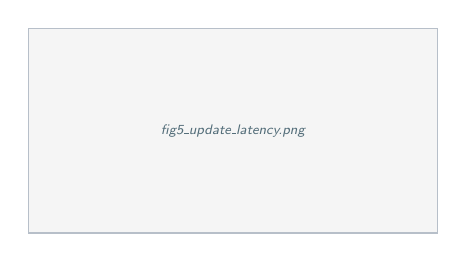
\begin{tikzpicture}
    \draw[fill=uhapGray,draw=uhapNavy!30] (0,0) rectangle (5.2,2.6);
    \node[font=\tiny\itshape,text=uhapGrayD] at (2.6,1.3)
      {fig5\_update\_latency.png};
  \end{tikzpicture}%
}
\vspace{2pt}
\begin{callout}[fontupper=\scriptsize]{Key Results}
\begin{itemize}\tightitems
\item \textbf{2.73$\times$ faster} total update at $n{=}2{,}000$ (223\,ms vs.\ 611\,ms)
\item \textbf{19.5$\times$ faster} post-parse engine path at $n{=}2{,}000$
\item U-HAP grows linearly; OPA grows super-linearly
\item 100/100 decisions verified identical (equiv.\ gate)
\end{itemize}
\end{callout}
\end{column}
%% Right: vertical table
\begin{column}{0.43\textwidth}
{\tiny\textbf{Edit-to-first-decision latency (ms)}}
\vspace{3pt}
\setlength{\tabcolsep}{2pt}\renewcommand{\arraystretch}{1.15}
\begin{tabular}{@{}r rr c rr@{}}
\toprule
\tiny & \multicolumn{2}{c}{\tiny\textbf{Total (ms)}} & & \multicolumn{2}{c}{\tiny\textbf{Post-parse (ms)}} \\
\cmidrule(lr){2-3}\cmidrule(lr){5-6}
\tiny $n$ & \tiny U-HAP & \tiny OPA & \tiny $\times$ & \tiny U-HAP & \tiny OPA \\
\midrule
\tiny 10   & \tiny 1.75   & \tiny 2.85   & \tiny 1.63 & \tiny 0.14  & \tiny 2.85 \\
\tiny 100  & \tiny 14.76  & \tiny 26.60  & \tiny 1.80 & \tiny 2.03  & \tiny 26.60 \\
\tiny 500  & \tiny 57.35  & \tiny 119.40 & \tiny 2.08 & \tiny 7.87  & \tiny 119.40 \\
\tiny 1000 & \tiny 109.99 & \tiny 277.32 & \tiny 2.52 & \tiny 16.27 & \tiny 277.32 \\
\tiny\bfseries 2000 & \tiny\bfseries 223.41 & \tiny\bfseries 610.54 & \tiny\bfseries 2.73 & \tiny\bfseries 31.31 & \tiny\bfseries 610.54 \\
\bottomrule
\end{tabular}
\end{column}
\end{columns}
\end{frame}

% ════════════════════════════════════════════════════════════════════════════
% 11. CONCLUSION
% ════════════════════════════════════════════════════════════════════════════
\begin{frame}[t]{Conclusion}
\vspace{3pt}
\begin{columns}[T,onlytextwidth]
\begin{column}{0.49\textwidth}
\begin{callout}[fonttitle=\bfseries\small,fontupper=\scriptsize]{What We Built}
U-HAP is a \textbf{compilation-driven, index-based} Kubernetes webhook
authorizer unifying RBAC, ABAC, and ACL under a single semantic DAG with
deterministic deny-override conflict resolution.
\end{callout}
\vspace{3pt}
\begin{callout}[fonttitle=\bfseries\scriptsize]{Key Results}
\begin{itemize}\tightitems
\item \textbf{Near-constant latency}: ${\approx}1.7\times$ vs.\ SSO; flat to $N{=}1{,}000$ namespaces
\item \textbf{${\sim}14\times$ caching speedup} on repeated requests
\item \textbf{16.9$\times$ ABAC speedup} at $k{=}320$; RBAC $5.6\times$, ACL $5.0\times$
\item \textbf{2.73$\times$ faster} policy-update vs.\ OPA at $n{=}2{,}000$
\item \textbf{19.5$\times$ faster} post-parse path vs.\ OPA
\end{itemize}
\end{callout}
\end{column}
\begin{column}{0.49\textwidth}
\begin{callout}[fonttitle=\bfseries\scriptsize]{Why It Works}
\begin{itemize}\tightitems
\item \textbf{Compile, don't scan} --- all complexity offline; runtime is index lookup + bitwise ops only
\item \textbf{Share, don't repeat} --- hash consing eliminates redundant sub-expression evaluation
\item \textbf{Prune early, prune deep} --- two-level pruning skips entire model classes before eval
\end{itemize}
\end{callout}
\vspace{3pt}
\begin{callout}[fonttitle=\bfseries\scriptsize]{Future Work}
\begin{itemize}\tightitems
\item Reimplement in Go/Rust to eliminate Python/Gunicorn HTTP overhead
\item Cross-namespace policy composition
\item Dynamic policy reload without restart
\end{itemize}
\end{callout}
\end{column}
\end{columns}
\end{frame}

% ════════════════════════════════════════════════════════════════════════════
% 11b. REFERENCES  (slide before last)
% ════════════════════════════════════════════════════════════════════════════
\begin{frame}[t]{References}
\vspace{2pt}
\begin{columns}[T,onlytextwidth]
\begin{column}{0.49\textwidth}
{\tiny\setlength{\parindent}{0pt}\setlength{\parskip}{2.2pt}%
\everypar{\hangindent=1.0em\hangafter=1}%
[1] NSA \& CISA, ``Kubernetes Hardening Guidance,'' NSA Cybersec.\ Tech.\ Report, ver.\ 1.2, 2022.\par
[2] A.\ Rahman \emph{et al.}, ``Security Misconfigurations in Open Source Kubernetes Manifests,'' \emph{ACM TOSEM}, 32(4), 2023.\par
[3] N.\ Yang \emph{et al.}, ``Take Over the Whole Cluster: Attacking Kubernetes via Excessive Permissions,'' \emph{ACM CCS}, 2023.\par
[4] G.\ Rostami, ``RBAC Authorization in Kubernetes,'' \emph{J.\ ICT Standardization}, 11(3), 2023.\par
[5] N.\ Farhadighalati \emph{et al.}, ``A Systematic Review of Access Control Models,'' \emph{IEEE Access}, 13, 2025.\par
[6] M.\ S.\ Rahaman \emph{et al.}, ``Access Control in Cloud-Native Architecture: A Mapping Study,'' \emph{Sensors}, 23(7), 2023.\par
[7] OASIS, ``XACML Version 3.0 Plus Errata 01,'' OASIS Standard, 2017.\par
[8] M.\ Yang \emph{et al.}, ``A Graph-Based Framework for ABAC Policy Enforcement and Analysis,'' \emph{DBSec}, 2024.\par
[9] Z.\ Mori\'c \emph{et al.}, ``Security Hardening and Compliance Assessment of Kubernetes,'' \emph{J.\ Cybersec.\ Privacy}, 5(2), 2025.\par
}
\end{column}
\begin{column}{0.49\textwidth}
{\tiny\setlength{\parindent}{0pt}\setlength{\parskip}{2.2pt}%
\everypar{\hangindent=1.3em\hangafter=1}%
[10] Y.\ Gu \emph{et al.}, ``EPScan: Automated Detection of Excessive RBAC Permissions in Kubernetes,'' \emph{IEEE S\&P}, 2025.\par
[11] A.\ Sissodiya \emph{et al.}, ``Formal Verification for Preventing Misconfigured Access Policies in Kubernetes,'' \emph{IEEE Access}, 13, 2025.\par
[12] R.\ Chandramouli \& Z.\ Butcher, ``A Zero Trust Architecture Model for Cloud-Native Applications,'' \emph{NIST SP 800-207A}, 2023.\par
[13] H.\ Nguyen \emph{et al.}, ``PerfSPEC: Profiling-Based Proactive Security Policy Enforcement for Containers,'' \emph{IEEE Computer}, 2025.\par
[14] S.\ Kern \emph{et al.}, ``Optimization of Access Control Policies,'' \emph{J.\ Inf.\ Secur.\ Appl.}, 70, 2022.\par
[15] A.\ X.\ Liu \emph{et al.}, ``Designing Fast and Scalable XACML Policy Evaluation Engines,'' \emph{IEEE Trans.\ Computers}, 60(12), 2011.\par
[16] L.\ Ma \emph{et al.}, ``Authorization Model of Attribute Access Control Based on Knowledge Graph,'' \emph{UbiSec}, 2024.\par
[17] R.\ Pang \emph{et al.}, ``Zanzibar: Google's Consistent, Global Authorization System,'' \emph{USENIX ATC}, 2019.\par
[18] M.\ Davari \& M.\ Zulkernine, ``Automatic Conversion of ABAC Policies for RBAC Systems,'' \emph{IEEE DSC}, 2023.\par
}
\end{column}
\end{columns}
\end{frame}

% ════════════════════════════════════════════════════════════════════════════
% 12. THANK YOU  (final slide)
% ════════════════════════════════════════════════════════════════════════════
{\setbeamertemplate{footline}{}
\begin{frame}[plain,noframenumbering]
\dividerBg
\vbox to \textheight{\vfil
  \hbox to \textwidth{\hfil
    \fontsize{38pt}{42pt}\selectfont\bfseries\color{white}Thank you!\hfil}%
  \vskip 12pt
  \hbox to \textwidth{\hfil
    \large\color{white!85!black}Questions are welcome.\hfil}%
  \vskip 16pt
  \hbox to \textwidth{\hfil
    \small\color{uhapTeal}
    \begin{tabular}{l}
    Singha Junchan --- \texttt{6622770350@g.siit.tu.ac.th}\\
    School of ICT, SIIT, Thammasat University
    \end{tabular}\hfil}%
  \vfil}
\end{frame}}

% ════════════════════════════════════════════════════════════════════════════
% BACKUP SLIDES
% ════════════════════════════════════════════════════════════════════════════

% ── B1. Runtime Evaluation Order ────────────────────────────────────────────
\begin{frame}[t,noframenumbering]{Backup: Runtime Evaluation Order (Phase 3)}
\vspace{3pt}
\begin{columns}[T,onlytextwidth]
\begin{column}{0.54\textwidth}
\begin{callout}{Evaluation Pipeline for each SAR}
\begin{enumerate}\tightitems
\item \textbf{Cache hit?} Return cached decision immediately
\item \textbf{Deny check}: token-pruned candidates from $I^{\mathrm{deny}}$; any match $\Rightarrow$ \texttt{DENY}
\item \textbf{ACL}: $\mathrm{uid} \in I_{\mathrm{acl}}$ or $\mathrm{groups} \cap I_{\mathrm{acl}} \neq \emptyset$ (hash set, O(1))
\item \textbf{RBAC}: $b_{\mathrm{user}}\ \&\ b_{\mathrm{rbac}} \neq 0$ (one bitwise AND)
\item \textbf{ABAC}: attribute-key pruned $\to$ cost-sorted $\to$ hash-consed gate eval
\item \textbf{Default Deny}: no rule matched $\Rightarrow$ \texttt{DENY}
\end{enumerate}
\end{callout}
\end{column}
\begin{column}{0.44\textwidth}
\begin{callout}{Correctness Invariants}
\begin{itemize}\tightitems
\item \textbf{Deny-overrides-all} checked first, always
\item \textbf{DAG acyclicity} verified at compile time
\item \textbf{Resource-action isolation}: eval of $(n,r,a)$ touches only $C_{\langle n,r,a\rangle}$
\item \textbf{Deterministic}: same input $\Rightarrow$ same output
\item \textbf{Memoization}: each DAG node evaluated at most once per request
\item \textbf{Cache consistency}: invalidated on any policy change
\end{itemize}
\end{callout}
\end{column}
\end{columns}
\end{frame}

% ── B2. Scenarios S1–S7 ──────────────────────────────────────────────────────
\begin{frame}[t,noframenumbering]{Backup: Correctness Scenarios S1--S7}
\vspace{4pt}
\centering
\setlength{\tabcolsep}{5pt}
\renewcommand{\arraystretch}{1.3}
\begin{tabular}{c l l l l c}
\toprule
\rowcolor{uhapGray}
\tiny\textbf{ID} & \tiny\textbf{Subject} & \tiny\textbf{Model} &
\tiny\textbf{Resource / Verb} & \tiny\textbf{Context} & \tiny\textbf{Expected} \\
\midrule
\tiny S1 & \tiny alice   & \tiny ABAC      & \tiny pods/prod / get    & \tiny on-premise + business-hours & \tiny\bfseries\color{uhapGreen}ALLOW \\
\tiny S2 & \tiny alice   & \tiny ABAC      & \tiny pods/prod / get    & \tiny remote                      & \tiny\bfseries\color{uhapRed}DENY \\
\tiny S3 & \tiny alice   & \tiny RBAC      & \tiny pods/dev / get     & \tiny any                         & \tiny\bfseries\color{uhapGreen}ALLOW \\
\tiny S4 & \tiny bob     & \tiny ABAC      & \tiny pods/prod / delete & \tiny after-hours                 & \tiny\bfseries\color{uhapRed}DENY \\
\tiny S5 & \tiny *       & \tiny Deny      & \tiny secrets / delete   & \tiny any                         & \tiny\bfseries\color{uhapRed}DENY \\
\tiny S6 & \tiny charlie & \tiny ACL       & \tiny pods/dev / get     & \tiny any                         & \tiny\bfseries\color{uhapGreen}ALLOW \\
\tiny S7 & \tiny dave    & \tiny Hierarchy & \tiny pods/prod / get    & \tiny any                         & \tiny\bfseries\color{uhapGreen}ALLOW \\
\bottomrule
\end{tabular}\\[5pt]
{\tiny\color{uhapGrayD}S7: dave is a Senior Developer. RBAC bit-vector encodes full transitive role closure at compile time --- no runtime BFS needed.}\\[4pt]
\highlightbanner{All 7 scenarios are non-negotiable correctness gates. All pass in the U-HAP implementation.}
\end{frame}

% ── B3. Hash Consing Example ─────────────────────────────────────────────────
\begin{frame}[t,noframenumbering]{Backup: Hash Consing --- Worked Example (P1--P4)}
\vspace{3pt}
\begin{columns}[T,onlytextwidth]
\begin{column}{0.49\textwidth}
\begin{callout}{Without Hash Consing (Na\"ive Tree)}
Four policies P1--P4 share the predicate
\texttt{time.hour $\in$ [9,18]} and \texttt{location = "on-premise"},
but each expands them independently.

Na\"ive tree: \textbf{11 nodes}.

The shared predicates are evaluated \emph{redundantly} for each policy, even within the same request.
\end{callout}
\end{column}
\begin{column}{0.49\textwidth}
\begin{callout}{With Hash Consing (DAG)}
Structural equality check at compile time identifies shared sub-expressions. One canonical node per unique predicate.

Hash-consed DAG: \textbf{8 nodes}.

At request time, each node is evaluated \emph{at most once} and its result memoized. Policies referencing the same predicate re-use the cached result --- zero redundant computation.
\end{callout}
\end{column}
\end{columns}
\vspace{4pt}
\highlightbanner{As policy sets grow and predicates are reused across rules, hash consing provides sub-linear growth in both DAG size and evaluation cost.}
\end{frame}

% ── B4. RBAC Bit-Vector ──────────────────────────────────────────────────────
\begin{frame}[t,noframenumbering]{Backup: RBAC Bit-Vector and Role Closure}
\vspace{3pt}
\begin{columns}[T,onlytextwidth]
\begin{column}{0.54\textwidth}
\begin{callout}{Compile-Time Transitive Closure}
Role hierarchy is a DAG (acyclicity checked at compile time).
Compiler computes full transitive closure for every role $r$:
\[ b_r = \bigl\{\,r' \mid r' \text{ is reachable from } r\,\bigr\} \]
encoded as a bit-vector. User's effective vector:
\[ b_{\mathrm{user}} = \bigvee_{r \in \mathrm{user.roles}} b_r \]
\end{callout}
\begin{callout}{Runtime RBAC Check}
Each $(n,r,a)$ artifact stores $b_{\mathrm{rbac}}$ --- roles allowed for this resource/action:
\[ \text{ALLOW} \iff b_{\mathrm{user}}\ \&\ b_{\mathrm{rbac}} \neq 0 \]
One bitwise AND. No graph traversal. Independent of rule count.
\end{callout}
\end{column}
\begin{column}{0.44\textwidth}
\begin{callout}{Why This Eliminates Linear Scan}
\begin{itemize}\tightitems
\item Traditional RBAC (SSO baseline): iterate roles + hierarchy traversal per request --- O(\#roles $\times$ \#rules), cost scales linearly with rule count
\item U-HAP at $k{=}320$ RBAC rules: \textbf{5.6$\times$} speedup vs.\ baseline
\item At $k{=}1{,}000$+: speedup continues to grow as baseline cost scales linearly
\end{itemize}
Hierarchy traversal cost is paid \emph{once} at compilation, not at every request.
\end{callout}
\end{column}
\end{columns}
\end{frame}

% ── B5. Decision Cache ───────────────────────────────────────────────────────
\begin{frame}[t,noframenumbering]{Backup: Decision Cache}
\vspace{3pt}
\begin{columns}[T,onlytextwidth]
\begin{column}{0.49\textwidth}
\begin{callout}{Cache Behavior}
\begin{itemize}\tightitems
\item Cache key: $(n, r, a, \mathrm{uid}, \mathrm{groups}, \mathrm{attributes})$
\item Cache hit returns stored ALLOW/DENY instantly
\item \textbf{Invalidated} on any policy change (compilation event)
\item Consistency invariant: stale decisions never served after policy update
\end{itemize}
\end{callout}
\end{column}
\begin{column}{0.49\textwidth}
\begin{callout}{Measured Cache Impact}
In-memory benchmark (1\,000 iterations, 50 warm-ups):

\textbf{$\approx$14$\times$ speedup} on repeated requests ---
cache bypasses all evaluation, returning the stored decision in one hash-table lookup.

Benefit compounds at scale: Exp1 shows the 14$\times$ factor
holds across $N=1{,}000$ namespaces.
\end{callout}
\end{column}
\end{columns}
\vspace{4pt}
\highlightbanner{The cache is most valuable when the webhook is co-located with the API server --- U-HAP is designed for exactly this deployment model.}
\end{frame}

% ── B6. Implementation Details ───────────────────────────────────────────────
\begin{frame}[t,noframenumbering]{Backup: Implementation Details}
\vspace{3pt}
\begin{columns}[T,onlytextwidth]
\begin{column}{0.49\textwidth}
\begin{callout}{Codebase}
\setlength{\tabcolsep}{3pt}
\renewcommand{\arraystretch}{1.1}
\begin{tabular}{@{}l l@{}}
\toprule
\tiny Component & \tiny Language \\
\midrule
\tiny DSL models + parser       & \tiny Python 3.11 \\
\tiny Graph builder + hash cons & \tiny Python 3.11 \\
\tiny Index compiler + registry & \tiny Python 3.11 \\
\tiny Pruning engine + evaluator& \tiny Python 3.11 \\
\tiny Webhook handler           & \tiny Flask 3.x + Gunicorn \\
\tiny Audit logger              & \tiny Python 3.11 \\
\bottomrule
\end{tabular}
\end{callout}
\end{column}
\begin{column}{0.49\textwidth}
\begin{callout}{Deployment and Scope}
\begin{itemize}\tightitems
\item Standard K8s \texttt{SubjectAccessReview} webhook
\item Deployment manifests in \texttt{deploy/}
\item Test suite: S1--S7 scenario tests, hash-consing gate, role-closure, evaluator unit tests
\end{itemize}
\vspace{2pt}
\textbf{Out of scope:}
\begin{itemize}\tightitems
\item Cross-namespace access / ClusterRole
\item Dynamic policy reload without restart
\item JWT validation / authentication
\end{itemize}
\end{callout}
\end{column}
\end{columns}
\end{frame}

% ── B7. Policy DSL Example ────────────────────────────────────────────────────
\begin{frame}[t,noframenumbering]{Backup: Policy DSL --- YAML Format}
\vspace{3pt}
\begin{columns}[T,onlytextwidth]
\begin{column}{0.53\textwidth}
\begin{callout}{Sample Policy File (namespace: prod, resource: pods)}
{\setlength{\parskip}{0pt}\setlength{\baselineskip}{9.5pt}%
\texttt{\tiny namespace: prod\hspace{6pt}resource: pods}\\
\texttt{\tiny rules:}\\
\texttt{\tiny\hspace{5pt}\# ABAC --- attribute conditions}\\
\texttt{\tiny\hspace{5pt}- type: abac\hspace{4pt}action: get}\\
\texttt{\tiny\hspace{7pt}\phantom{-}\,predicate: "net=='on-premise' AND}\\
\texttt{\tiny\hspace{22pt}time=='business-hours'"}\\[2pt]
\texttt{\tiny\hspace{5pt}\# RBAC --- role-based access}\\
\texttt{\tiny\hspace{5pt}- type: rbac\hspace{4pt}role: viewer\hspace{4pt}action: get}\\[2pt]
\texttt{\tiny\hspace{5pt}\# ACL --- direct user grant}\\
\texttt{\tiny\hspace{5pt}- type: acl\hspace{4pt}subject: charlie\hspace{4pt}action: get}\\[2pt]
\texttt{\tiny\hspace{5pt}\# Deny --- always evaluated first}\\
\texttt{\tiny\hspace{5pt}- type: deny\hspace{4pt}subject: "*"\hspace{4pt}action: deletecollection}\\[2pt]
\texttt{\tiny\hspace{5pt}\# Hierarchy --- role inheritance}\\
\texttt{\tiny\hspace{5pt}- type: hierarchy}\\
\texttt{\tiny\hspace{7pt}\phantom{-}\,parent: senior-dev\hspace{4pt}child: junior-dev}%
}
\end{callout}
\end{column}
\begin{column}{0.45\textwidth}
\begin{callout}{Five Rule Types}
\setlength{\tabcolsep}{3pt}\renewcommand{\arraystretch}{1.2}
\begin{tabular}{@{}>{\ttfamily\tiny\bfseries\color{uhapNavy}}l >{\tiny}p{4.0cm}@{}}
deny      & Hard block; checked first, overrides any allow \\
acl       & Direct uid/group grant; O(1) hash-set lookup \\
rbac      & Role-based; hierarchy compiled into bit-vector \\
abac      & Attribute predicate gate; hash-consed + cost-sorted \\
hierarchy & Role inheritance edge (parent $\to$ child) \\
\end{tabular}
\end{callout}
\vspace{3pt}
\begin{callout}{Compiled Artifacts $C_{\langle n,r,a\rangle}$}
\setlength{\tabcolsep}{3pt}\renewcommand{\arraystretch}{1.15}
\begin{tabular}{@{}>{\tiny\bfseries\color{uhapTeal}}l >{\tiny}p{3.5cm}@{}}
$I_{\mathrm{deny}}$ & Deny candidate set (token-pruned hash set) \\
$I_{\mathrm{acl}}$  & ACL uid + group hash set \\
$b_{\mathrm{rbac}}$ & RBAC transitive-closure bit-vector \\
$I_{\mathrm{abac}}$ & ABAC gate list, cost-sorted \\
\end{tabular}
\end{callout}
\end{column}
\end{columns}
\end{frame}

% ── B8. System Comparison ─────────────────────────────────────────────────────
\begin{frame}[t,noframenumbering]{Backup: System Comparison}
\vspace{5pt}
\centering
\setlength{\tabcolsep}{3pt}
\renewcommand{\arraystretch}{1.5}
\begin{tabular}{@{}>{\tiny\bfseries}p{3.6cm} >{\centering\tiny}p{2.1cm} >{\centering\tiny}p{2.0cm} >{\centering\tiny}p{1.9cm} >{\centering\arraybackslash\tiny}p{2.3cm}@{}}
\toprule
\rowcolor{uhapGray}
\textbf{Feature} & \textbf{U-HAP} & \textbf{K8s RBAC} & \textbf{OPA} & \textbf{Keycloak 24} \\
\midrule
Multi-model support
  & \textbf{\color{uhapGreen}RBAC+ABAC+\allowbreak ACL+Deny}
  & RBAC only
  & Policy-defined
  & RBAC+group+user \\
Deny-overrides-all guarantee
  & \textbf{\color{uhapGreen}Always, enforced}
  & Not explicit
  & Policy-defined
  & Not explicit \\
Compile-time indexing
  & \textbf{\color{uhapGreen}Full}
  & No
  & Partial (Rego partial eval)
  & No \\
Request-time complexity
  & \textbf{\color{uhapGreen}O(1) lookup}
  & O(rules)
  & O(rules)
  & O(rules) \\
K8s SAR webhook
  & \textbf{\color{uhapGreen}Native}
  & Built-in
  & Via adapter
  & Via adapter \\
Rule-density speedup (RBAC)
  & \textbf{\color{uhapGreen}5.6$\times$ at $k{=}320$}
  & ---
  & ---
  & linear scan \\
\bottomrule
\end{tabular}
\end{frame}

% ── B9. Limitations and Future Work ──────────────────────────────────────────
\begin{frame}[t,noframenumbering]{Backup: Limitations and Future Work}
\vspace{3pt}
\begin{columns}[T,onlytextwidth]
\begin{column}{0.49\textwidth}
\begin{callout}{Current Limitations}
\begin{itemize}\tightitems
\item \textbf{Single-namespace}: no cross-namespace access or \texttt{ClusterRole} support
\item \textbf{Restart to reload}: policy updates require webhook restart; hot-reload is not implemented
\item \textbf{Authorization only}: JWT/OIDC authentication is out of scope
\item \textbf{Simple deny predicates}: deny rules match on subject+action only, not attribute conditions
\item \textbf{Single-process}: no multiprocessing (ThreadPoolExecutor used for batch evaluation only)
\end{itemize}
\end{callout}
\end{column}
\begin{column}{0.49\textwidth}
\begin{callout}{Future Directions}
\begin{itemize}\tightitems
\item \textbf{Cluster scope}: extend $C_{\langle n,r,a\rangle}$ to \texttt{ClusterRole} and cross-namespace policies
\item \textbf{Incremental compilation}: re-compile only affected $(n,r,a)$ artifacts on policy edit
\item \textbf{Conditional deny}: ABAC-style attribute predicates inside deny rules
\item \textbf{gRPC / Unix socket}: lower-latency transport for co-located deployment
\item \textbf{Formal verification}: prove deny-overrides invariant holds for all valid DSL inputs
\end{itemize}
\end{callout}
\end{column}
\end{columns}
\end{frame}

\end{document}
